\documentclass[10pt]{article}
\usepackage[vietnamese]{babel}
\usepackage[utf8]{inputenc}
\usepackage[T5]{fontenc}
\usepackage{amsmath}
\usepackage{amsfonts}
\usepackage{amssymb}
\usepackage[version=4]{mhchem}
\usepackage{stmaryrd}
\usepackage{graphicx}
\usepackage[export]{adjustbox}
\graphicspath{ {./images/} }

\begin{document}
\section*{Phoin II \\
 DAP AN VA TU'ONG DÍN GIẢ}
\section*{Chưong I ESTER - LIPID}
\section*{BAI 1 ESTER - LIPID}
\begin{center}
\begin{tabular}{lllll}
1.1. A & $1.2 . \mathrm{A}$ & $1.3 . \mathrm{D}$ & $1.4 . \mathrm{A}$ & $1.5 . \mathrm{C}$ \\
$1.6 . \mathrm{B}$ & $1.7 . \mathrm{A}$ & $1.8 . \mathrm{D}$ & $1.9 . \mathrm{A}$ & $1.10 . \mathrm{D}$ \\
$1.11 . \mathrm{A}$ & $1.12 . \mathrm{C}$ & $1.13 . \mathrm{D}$ & $1.14 . \mathrm{B}$ & $1.15 . \mathrm{C}$ \\
$1.16 . \mathrm{B}$ & $1.17 . \mathrm{C}$ & $1.18 . \mathrm{B}$ & $1.19 . \mathrm{B}$ & $1.24 . \mathrm{C}$ \\
\end{tabular}
\end{center}

1.20. a) - đúng; b) - đúng; c) - sai; d) - đúng.\\
1.21. a) - đúng; b) - sai; c) - sai; d) - đúng.\\
1.22. a) - sai; b) - đứng; c) - sai; d) - đúng.\\
1.23. $\mathrm{n}_{\mathrm{CH}_{3} \mathrm{COOC}_{2} \mathrm{H}_{5}}=\frac{4,4}{88}=0,05(\mathrm{~mol})$.

$$
\begin{aligned}
& \mathrm{CH}_{3} \mathrm{COOC}_{2} \mathrm{H}_{5}+\mathrm{NaOH} \longrightarrow \mathrm{CH}_{3} \mathrm{COONa}+\mathrm{C}_{2} \mathrm{H}_{5} \mathrm{OH} \\
& \mathrm{n}_{\mathrm{CH}_{3} \mathrm{COONa}}=\mathrm{n}_{\mathrm{CH}_{3} \mathrm{COOC}_{2} \mathrm{H}_{5}}=0,05(\mathrm{~mol}) . \\
& \mathrm{m}_{\mathrm{CH}_{3} \mathrm{COONa}}=0,05 \cdot 82=4,1(\mathrm{~g}) .
\end{aligned}
$$

1.25. a) - đúng; b) - sai; c) - sai; d) - sai.\\
1.26. a) - đúng; b) - đúng; c) - sai; d) - sai.\\
1.27. $\mathrm{m}_{\text {ester }}=0,067 \cdot 102=6,834(\mathrm{~g})$.\\
1.28. Giả sử lấy 1 g chất béo có $0,65 \mathrm{~g}$ tristearin và $0,23 \mathrm{~g}$ triolein.

$$
\begin{aligned}
& \mathrm{n}_{\mathrm{KOH}}=3 \cdot\left(\mathrm{n}_{\text {tristearin }}+\mathrm{n}_{\text {triolein }}\right)=2,97 \cdot 10^{-3}(\mathrm{~mol}) . \\
& \mathrm{m}_{\mathrm{KOH}}=2,97 \cdot 10^{-3} \cdot 56=166,3 \cdot 10^{-3}(\mathrm{~g})=166,3(\mathrm{mg}) .
\end{aligned}
$$

1.29.\\
a)\\
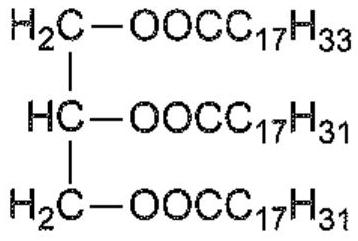
\includegraphics[max width=\textwidth, center]{2025_10_23_b82d44049ffb48e891e8g-02(1)}\\
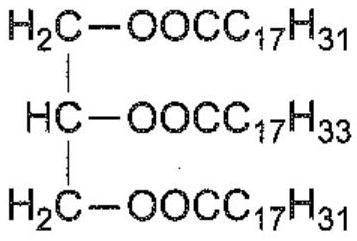
\includegraphics[max width=\textwidth, center]{2025_10_23_b82d44049ffb48e891e8g-02}\\
b)\\
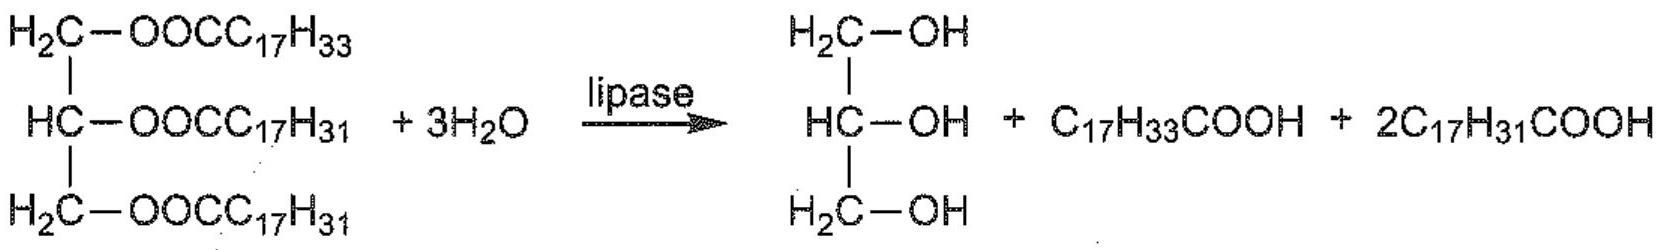
\includegraphics[max width=\textwidth, center]{2025_10_23_b82d44049ffb48e891e8g-02(3)}\\
c)\\
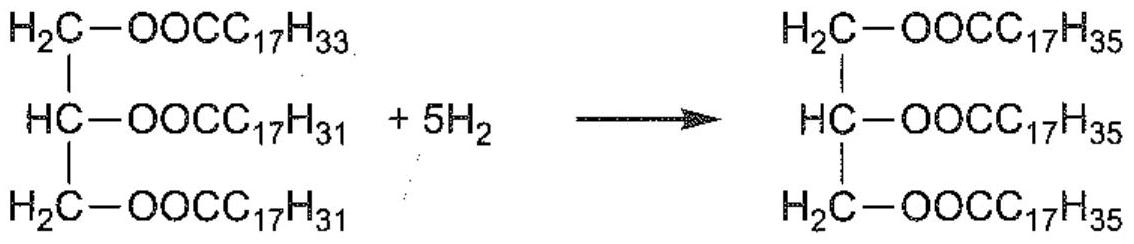
\includegraphics[max width=\textwidth, center]{2025_10_23_b82d44049ffb48e891e8g-02(2)}

\section*{BÀ1 2. XÀ PHÒNG VÀ CHẤT GIẠT RỬA}
2.1. D\\
2.2. B\\
2.3. C\\
2.4. C\\
2.5. A\\
2.6. D\\
2.7. C\\
2.8. D\\
2.9. D\\
2.10. C\\
2.13. C\\
2.11. a) - đúng; b) - sai; c) - sai; d) - đúng.\\
2.12. a) - đúng; b) - đúng; c) - sai; d) - đúng.\\
2.14, a) - sai; b) - sai; c) - đúng; d) - đúng.\\
2.15. a) - sai; b) - đúng; c) - đúng; d) - đúng.\\
2.16. a) $\left(\mathrm{C}_{17} \mathrm{H}_{35} \mathrm{COO}\right)_{3} \mathrm{C}_{3} \mathrm{H}_{5}+3 \mathrm{NaOH} \longrightarrow \mathrm{C}_{3} \mathrm{H}_{5}(\mathrm{OH})_{3}+\mathrm{C}_{17} \mathrm{H}_{35} \mathrm{COONa}$

NaOH hoà tan vào nước và toả nhiệt làm cho phản ứng xà phòng hoá xảy ra dễ hơn. Xà phòng tạo thành tan được trong nước làm cho đường ống không bị tắc.\\
b) $\mathrm{M}_{\text {tristearin }}=890$.

Ta có: $\mathrm{n}_{\mathrm{NaOH}}=0,3 \mathrm{~mol}$.\\
$\Rightarrow \mathrm{n}_{\text {tristearin }}=\frac{1}{3} \cdot \mathrm{n}_{\mathrm{NaOH}}=0,1(\mathrm{~mol})$.\\
$\Rightarrow \mathrm{m}_{\text {tristearin }}=0,3 \cdot 890=267(\mathrm{~g})$.\\
2.17. $\mathrm{M}_{\text {stearic acid }}=284 ; \mathrm{M}_{\text {tristearin }}=890$.

Trong 1 g chất béo có:\\
$\mathrm{n}_{\text {stearic acid }}=1,25.10^{-4} \mathrm{~mol} ; \mathrm{n}_{\text {tristearin }}=0,001 \mathrm{~mol}$.\\
$\mathrm{n}_{\mathrm{KOH} \text { phản ứng }}=1,25 \cdot 10^{-4}+3 \cdot 0,001=0,003125(\mathrm{~mol})$.\\
$\mathrm{m}_{\mathrm{KOH}}=0,003125 \cdot 56=0,175(\mathrm{~g})=175 \mathrm{mg}$.\\
$\Rightarrow$ Chỉ số xà phòng hoá của chất béo đó là 175 .

\section*{BAI 3. ÔN TẬP CHƯƠNG I}
\begin{center}
\begin{tabular}{llll}
3.1. A & 3.2. C & 3.3. C & 3.4. D \\
3.5. B & 3.6. D & 3.7. B &  \\
3.8. D & 3.9. B & 3.10. B &  \\
3.14. C & 3.15. A & 3.16. C &  \\
\end{tabular}
\end{center}

3.11. a) - sai; b) - sai; c) - đúng; d) - sai.\\
3.12. a) - đúng; b) - sai; c) - đúng; d) - đúng.\\
3.13.\\
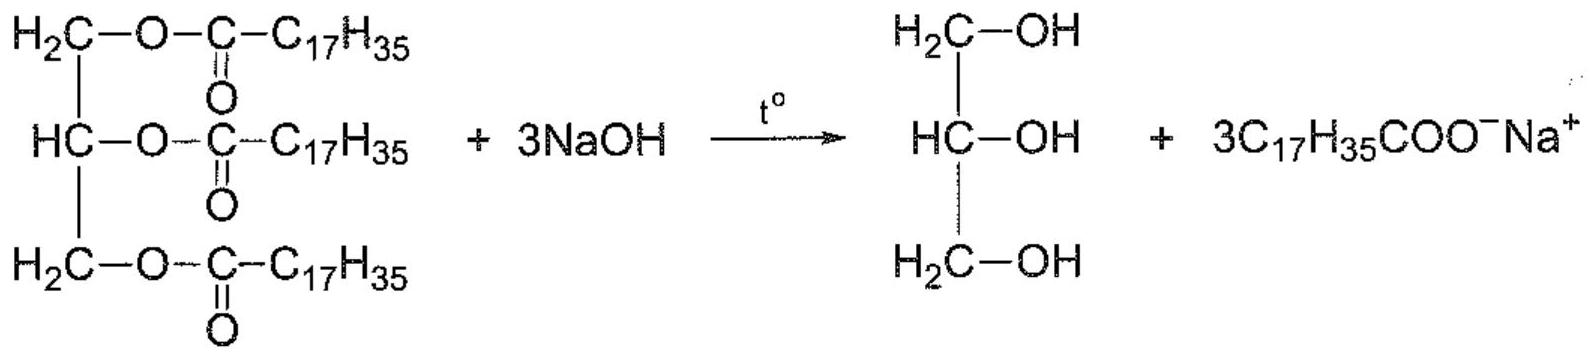
\includegraphics[max width=\textwidth, center]{2025_10_23_b82d44049ffb48e891e8g-03}

Ta có: $\mathrm{n}_{\text {stearin }}=\frac{80 \cdot 10^{3}}{890}=89,888(\mathrm{~mol})$.\\
$\Rightarrow \mathrm{n}_{\text {xà phòng }}=89,888 \cdot 3=269,66(\mathrm{~mol})$.\\
Do hiệu suất phản ứng là $90 \%$ nên khối lượng xà phòng tạo thành là:\\
$\mathrm{m}_{\text {sodium stearate }}=\frac{269,66 \cdot 306 \cdot 90}{100}=74,264(\mathrm{~kg})$.\\
3.17. Số mol chất béo $=0,005 \mathrm{~mol}=\mathrm{n}_{\text {glycerol }}=3 \mathrm{n}_{\mathrm{NaOH}}$.

$$
\begin{aligned}
& \begin{array}{l}
\Rightarrow \mathrm{m}_{\text {muối }}=\mathrm{m}_{\text {chất béo }}+\mathrm{m}_{\mathrm{NaOH}}-\mathrm{m}_{\text {glycerol }}=4,42+0,015 \cdot 40-0,005 \cdot 92 \\
=4,56(\mathrm{~g}) .
\end{array} \\
& \begin{aligned}
\left(\mathrm{C}_{17} \mathrm{H}_{33} \mathrm{COO}\right)_{3} \mathrm{C}_{3} \mathrm{H}_{5}+3 \mathrm{H}_{2} \longrightarrow\left(\mathrm{C}_{17} \mathrm{H}_{35} \mathrm{COO}\right)_{3} \mathrm{C}_{3} \mathrm{H}_{5}
\end{aligned} \\
& \mathrm{n}_{\mathrm{H}_{2}}=3 \mathrm{n}_{\text {chất béo }}=0,015(\mathrm{~mol}) \\
& \Rightarrow \mathrm{V}_{\mathrm{H}_{2}}=0,015 \cdot 24,79 \approx 0,372 \text { (lít). }
\end{aligned}
$$

3.18. Công thức cấu tạo của chất béo: $\left(\mathrm{C}_{17} \mathrm{H}_{31} \mathrm{COO}\right)_{2}\left(\mathrm{C}_{17} \mathrm{H}_{33} \mathrm{COO}\right) \mathrm{C}_{3} \mathrm{H}_{5}$.\\
$\mathrm{M}_{\text {chất béo }}=880$.\\
Giả sử lấy 1 g dầu hướng dương có $0,88 \mathrm{~g}$ chất béo $\Rightarrow \mathrm{n}_{\text {chất }}$ béo $=0,001(\mathrm{~mol})$.

$$
\begin{aligned}
& \mathrm{n}_{\mathrm{KOH}}=3 \cdot \mathrm{n}_{\text {chất béo }}=0,003(\mathrm{~mol}) . \\
& \mathrm{m}_{\mathrm{KOH}}=0,003 \cdot 56=168 \cdot 10^{-3}(\mathrm{~g})=168 \mathrm{mg} .
\end{aligned}
$$

Vậy, chỉ số ester hoá của dầu hướng dương là 168 .\\
3.19. a)

\begin{center}
\begin{tabular}{|l|l|l|l|l|}
\hline
Thure ãn nhanh (suât) & Tồng năng lurong (kcal) & Tông số chát béo (g) & Năng lương đóng góp bớ chât béo (kcal) & \% nang lưong do chất béo đóng góp \\
\hline
Thịt gà chiên rán & 830 & 46 & 414 & 50 \\
\hline
Bánh mì kẹp phô mai & 520 & 29 & 261 & 50 \\
\hline
Bánh mì kep hamburger & 254 & 7 & 63 & 25 \\
\hline
Bánh pizza & 560 & 18 & 162 & 29 \\
\hline
Khoai tây chiên & 279 & 13 & 117 & 42 \\
\hline
Một chiếc xúc xích cỡ lớn & 180 & 18 & 162 & 90 \\
\hline
\end{tabular}
\end{center}

b) Xúc xích có tỉ lệ \% chất béo đóng góp nhiều nhất vào tổng năng lượng của thức ăn.\\
c) Thịt gà chiên rán, bánh mì kẹp phô mai, khoai tây chiên, xúc xích cỡ lớn là các thức ăn dư thừa chất béo, có thể gây nên bệnh béo phì.

\section*{Churong II CARBOHYDRATE}
\section*{BAI 4. GIÓI THIỆU VỀ CARBOHYDRATE, GLUCOSE VÀ FRUCTOSE}
4.1. C\\
4.2. A

\begin{itemize}
  \item 4.3. B\\
4.4. C\\
4.5. C\\
4.6. D\\
4.7. D\\
4.8. A\\
4.9. A\\
4.10. B\\
4.11. a) - đúng; b) - sai; c) - đúng; d) - đúng.\\
4.12. a) - đúng; b) - đúng; c) - sai; d) - sai.\\
4.13. a) - sai; b) - đúng; c) - sai; d) - đúng.\\
4.14. a) - đúng; b) - sai; c) - đúng; d) - đúng.\\
4.15. a) - đúng; b) - đúng; c) - đúng; d) - đúng.\\
4.16. Glucose là một aldohexose chứa nhóm chức aldehyde, trong khi fructose là một ketohexose chứa nhóm chức ketone.\\
4.17. Thực phẩm tự nhiên giàu glucose gồm một số loại trái cây như chuối, nho và dưa hấu. Thực phẩm tự nhiên giàu fructose gồm một số loại trái cây như táo, lê, măng cụt, xoài và mật ong.\\
4.18. Khối lượng mẫu nước cam $=250 \cdot 1,05=262,5(\mathrm{~g})$.
\end{itemize}

Khối lượng fructose $=262,5 \cdot 2,5 \% \approx 6,56(\mathrm{~g})$.\\
Khối lượng glucose $=262,5 \cdot 2 \% \approx 5,25(\mathrm{~g})$.\\
4.19. Ethanol là sản phẩm chính trong phản ứng lên men rượu của glucose. Quá trình này được sử dụng trong việc sản xuất rượu vang, bia,...\\
4.20. Methyl $\alpha$-glucoside và methyl $\beta$-glucoside không còn nhóm -OH hemiacetal nên không có dạng mạch hở chứa nhóm aldehyde $\Rightarrow$ không phản ứng với thuốc thử Tollens.\\
4.21. Glucose là nguồn năng lượng chính cho các tế bào vì nó dễ dàng được chuyển hoá trong quá trình hô hấp tế bào để sản xuất ATP , một dạng năng lượng mà tế bào có thể sử dụng. Glucose có thể được phân giải nhanh chóng và hiệu quả\\
trong các điều kiện khác nhau, cung cấp năng lượng cần thiết cho các hoạt động cơ bản của cơ thể.\\
4.22. Trong y tế, glucose thường được dùng trong các dung dịch truyền để bổ sung năng lượng nhanh cho bệnh nhân.\\
Trong thể thao, glucose thường được dùng để bổ sung năng lượng nhanh cho vận động viên, giúp họ phục hồi sức lực một cách nhanh chóng.\\
4.23. Phương trình hoá học:\\
$\mathrm{C}_{6} \mathrm{H}_{12} \mathrm{O}_{6}+2\left[\mathrm{Ag}\left(\mathrm{NH}_{3}\right)_{2}\right] \mathrm{OH} \rightarrow \mathrm{CH}_{2} \mathrm{OH}[\mathrm{CHOH}]_{4} \mathrm{COONH}_{4}+2 \mathrm{Ag}+3 \mathrm{NH}_{3}+\mathrm{H}_{2} \mathrm{O}$\\
Số $\mathrm{mol} \mathrm{Ag}=\frac{100 \cdot 0,5 \cdot 10^{-4} \cdot 10,49}{108}=0,4856 \cdot 10^{-3}(\mathrm{~mol})$.\\
Khối lượng glucose $=\frac{0,4856 \cdot 10^{-3} \cdot 180}{2}=0,044(\mathrm{~g})$.\\
4.24. Phương trình hoá học:

$$
\mathrm{C}_{6} \mathrm{H}_{12} \mathrm{O}_{6} \rightarrow 2 \mathrm{C}_{2} \mathrm{H}_{5} \mathrm{OH}+2 \mathrm{CO}_{2}
$$

Khối lượng ethanol $=\frac{500 \cdot 0,2 \cdot 2 \cdot 46}{1 \cdot 180}=51(\mathrm{~kg})$.\\
$\mathrm{m}_{\text {ethanol }}=\frac{500 \cdot 0,2 \cdot 2 \cdot 46}{1 \cdot 180}=51(\mathrm{~kg})$.

\section*{BAI 5 SACCHAROSE VÀ MALTOSE}
5.1. B\\
5.2. B\\
5.3. C\\
5.4. C\\
5.5. B\\
5.6. C\\
5.7. a) - sai; b) - đúng; c) - sai; d) - đúng.\\
5.8. a) - sai; b) - đúng; c) - đúng; d) - đúng.\\
5.9. a) - đúng; b) - đúng; c) - đúng; d) - đúng.\\
5.10. Dạng mạch hở của maltose chứa nhóm aldehyde nên maltose có thể phản ứng với thuốc thử Tollens hay dung dịch nước bromine. Saccharose chỉ tồn tại dạng mạch vòng, không chứa nhóm aldehyde.\\
5.11. Phản ứng thuỷ phân saccharose trong môi trường acid tạo glucose và fructose. Hai chất này phản ứng được với $\mathrm{Cu}(\mathrm{OH})_{2}$ trong dung dịch NaOH , đun nóng, tạo kết tủa đỏ gạch.

Phương trình hoá học:\\
$\mathrm{C}_{12} \mathrm{H}_{22} \mathrm{O}_{11}+\mathrm{H}_{2} \mathrm{O} \xrightarrow{\mathrm{H}^{+}} \mathrm{C}_{6} \mathrm{H}_{12} \mathrm{O}_{6}$ (glucose) $+\mathrm{C}_{6} \mathrm{H}_{12} \mathrm{O}_{6}$ (fructose)\\
$\mathrm{C}_{6} \mathrm{H}_{12} \mathrm{O}_{6}+2 \mathrm{Cu}(\mathrm{OH})_{2}+\mathrm{NaOH} \xrightarrow{\mathrm{t}^{\circ}} \mathrm{CH}_{2} \mathrm{OH}[\mathrm{CHOH}]_{4} \mathrm{COONa}+\mathrm{Cu}_{2} \mathrm{O}+3 \mathrm{H}_{2} \mathrm{O}$\\
5.12. Tiêu thụ nhiều saccharose và maltose trong chế độ ăn uống hằng ngày có thể tăng nguy cơ sâu răng do chúng cung cấp nguồn thức ăn chó vi khuẩn gây hại trong miệng và chuyển hoá thành acid gây hại cho men răng.\\
5.13. Đây là lời khuyên hợp lí vì:

Đường tinh chế được hấp thụ nhanh chóng vào máu, làm tăng đột biến lượng đường (glucose) trong máu. Do đó, cơ thể phải sản xuất insulin liên tục để hạ mức đường huyết, dẫn đến áp lực lên tuyến tuỵ và có thể gây ra tình trạng kháng insulin, là tiền thân của bệnh tiểu đường loại 2 . Đồng thời việc tiêu thụ đường tinh luyện quá nhiều cũng liên quan đến bệnh béo phì, bệnh tim mạch,...

Các loại đường tự nhiên như mật ong, đường có trong trái cây,... thường chứa các dưỡng chất bổ sung như vitamin, khoáng chất và chất xơ. Chất xơ đặc biệt quan trọng, giúp làm chậm quá trình hấp thụ đường, giảm tác động tiêu cực lên mức đường trong máu và giúp cải thiện sức khoẻ đường ruột.\\
5.14. Khối lượng mạch nha cần có $=\frac{10000}{0,8}=12500(\mathrm{~kg})$.

Số bao mạch nha cần nhập $=\frac{12500}{50}=250$ (bao).

\section*{BÂl 6 TINH BỘT VÀ CELLULOSE}
6.1. C\\
6.2. A\\
6.3. B\\
6.4. A\\
6.5. C\\
6.6. D\\
6.7. B\\
6.8. B\\
6.9. A\\
6.10. C\\
6.11. a) - đúng; b) - đúng; c) - sai; d) - đúng.\\
6.12. a) - đúng; b) - đúng; c) - đúng; d) - đúng.\\
6.13. a) - đúng; b) - sai; c) - đúng; d) - đúng.\\
6.14. a) - đúng; b) - sai; c) - đúng; d) - đúng.\\
6.15. a) - đúng; b) - đúng; c) - đúng; d) - đúng.\\
6.16. Cellulose không thể tiêu hoá bởi enzyme trong hệ tiêu hoá của người.

Con người thiếu enzyme cellulase cần thiết để phân giải liên kết $\beta$-1,4-glycoside trong cellulose, vì vậy cellulose hoạt động như một chất xơ không tiêu hoá trong chế độ ăn.\\
6.17. Cellulose là thành phần không thể thiếu trong cấu trúc tế bào thực vật, có vai trò quan trọng trong việc tạo nên thành tế bào của thực vật, cung cấp sức mạnh cơ học và bảo vệ cho tế bào.\\
6.18. Phương trình hoá học:

$$
\left(\mathrm{C}_{6} \mathrm{H}_{10} \mathrm{O}_{5}\right)_{\mathrm{n}}+\mathrm{nH}_{2} \mathrm{O} \rightarrow \mathrm{nC}_{6} \mathrm{H}_{12} \mathrm{O}_{6}
$$

Khối lượng glucose $=\frac{162 \cdot 80 \cdot 180 \mathrm{n}}{100 \cdot 162 \mathrm{n}}=144(\mathrm{~g})$.\\
6.19. Cấu trúc phấn nhánh của amylopectin tạo điều kiện cho enzyme tiêu hoá như amylase tiếp xúc dễ dàng hơn, làm tăng tốc độ tiêu hoá.\\
6.20. Bột mì chưa tinh bột, khi được nấu chín, tinh bột nở ra và trở nên dính, giúp kết dính các thành phần khác lại với nhau.\\
6.21. Quá trình chuyển hoá tinh bột thành ethanol bao gồm hai giai đoạn chính: thuỷ phân tinh bột thành glucose bằng enzyme amylase; sau đó glucose được lên men bằng các loại men tương ứng (zymas) đề tạo ra ethanol và $\mathrm{CO}_{2}$. Các enzyme đóng vai trò xúc tác cho các phản ứng thuỷ phân và lên men.\\
6.22. Sơ đồ phản ứng:

$$
\left(\mathrm{C}_{6} \mathrm{H}_{10} \mathrm{O}_{5}\right)_{\mathrm{n}} \rightarrow \mathrm{nC}_{6} \mathrm{H}_{12} \mathrm{O}_{6} \rightarrow 2 \mathrm{nC}_{2} \mathrm{H}_{5} \mathrm{OH}
$$

Khối lượng ethanol thu được $=\frac{1 \cdot 90 \cdot 92 \mathrm{n}}{100 \cdot 162 \mathrm{n}}=0,51$ (tấn).

\section*{BAI 7. ÔN TÂP CHUONG II}
\begin{center}
\begin{tabular}{llll}
7.1. B & 7.2. C & 7.3. D & 7.4. D \\
7.6. B & 7.7. A & 7.8. C & 7.5. B \\
7.9. D & 7.10. D &  &  \\
\end{tabular}
\end{center}

7.11. a) 3; b) 2 .\\
7.12. a) 4; b) 3 .

\subsection*{7.13.3.}
7.14. a) - đúng; b) - sai; c) - sai; d) - đúng.\\
7.15. a) - đúng; b) - sai; c) - sai; d) - đúng.\\
7.16. a) - đúng; b) - đúng; c) - đúng; d) -sai.\\
7.17. a) - đúng; b) - đúng; c) - đúng; d) -sai.\\
7.18. a) - đúng; b) - sai; c) - đúng; d) - đúng.\\
7.19. Glucose và saccharose tan tốt trong nước do có liên kết hydrogen mạnh với nước. Cellulose có cấu trúc $\beta$-1,4-glycoside tạo nên mạng lưới chặt chễ, kích thước lớn, hạn chế khảnăng tương tác với nước. Do đó, cellulose không tan trong nước.\\
7.20. Tinh bột và cellulose đều là polymer của glucose nhưng khác biệt về loại liên kết giữa các đơn vị glucose cấu thành. Trong phân tử tinh bột chưa liên kết $\alpha-1,4$-glycoside và $\alpha-1,6$-glycoside (trong amylopectin), tạo ra cấu trúc linh hoạt và dễ tiêu hoá. Trong phân tử cellulose chứa liên kết $\beta$-1,4-glycoside, tạo ra một cấu trúc rất chắc chẳn, không linh hoạt, khó tiêu hoá bởi enzyme của động vật, đóng vai trò là thành phần cấu trúc của thực vật.\\
7.21. Glucose được sử dụng để bổ sung năng lượng do khả năng hấp thụ nhanh vào máu, cung cấp năng lượng tức thì cho cơ bắp và não bộ. Điều này rất quan trọng cho vận động viên cần năng lượng nhanh chóng để duy trì hiệu suất.\\
Saccharose là chất làm ngọt chính trong ngành công nghiệp thực phẩm do vị ngọt cao, ổn định dưới nhiệt độ cao và dễ kết hợp với các thành phần khác. Saccharose tạo cảm giác ngon miệng và được sử dụng rộng rãi trong sản xuất thực phẩm và đồ uống.\\
Hiệu quả năng lượng và tác động đến sức khoẻ:\\
Glucose cung cấp năng lượng nhanh nhưng cũng có thể dẫn đến sự biến động của đường huyết nếu tiêu thụ không kiểm soát. Saccharose khi được tiêu hoá thuỷ phân thành glucose và fructose, có thể cung cấp năng lượng bền vững hơn nhưng tiêu thụ quá mức có thể gây tăng cân, bệnh tiểu đường và các vấn đề sức khoẻ khác. Vì vậy, việc sử dụng chúng cần hợp lí để đảm bảo sức khoẻ.\\
7.22. Do các tính chất như tan trong nước nóng tạo hệ keo, tạo nguồn năng lượng trực tiếp (glucose) khi bị thuỷ phân,... nên tinh bột được ứng dụng rộng rãi trong công nghiệp thực phẩm (chất làm đặc, chất kết dính, sản xuất ethanol,...).

Ngoài ra, tinh bột cũng được sử dụng làm chất kết dính trong công nghiệp giấy và công nghiệp dệt may.\\
Do cấu trúc dạng sợi, dài mảnh bền và có khả năng tái chế, cellulose được ứng dụng phổ biến trong sản xuất giấy và bao bì. Ngoài ra, cellulose cũng được sử dụng làm tơ sợi tự nhiên và nhân tạo.

\section*{Churong III HOP CHÁT CHÚA NITROGEN}
\section*{BAI 8 AMINE}
8.1. B\\
8.2. C\\
8.3. D\\
8.4. B\\
8.5. A\\
8.6. A\\
8.7. B\\
8.8. A\\
8.9. C\\
8.10. D\\
8.11. a) - đúng; b) - sai; c) - sai; d) - dúng.\\
8.12. a) - đúng; b) - đúng; c) - đúng; d) - đúng.\\
8.13. a) - sai; b) - đúng; c) - đúng; d) - đúng.\\
8.14. a) - đúng; b) - đúng; c) - đúng; d) - sai.\\
8.15. a) - đúng; b) - đúng; c) - đúng; d) - đúng.\\
8.16. Phương trình hoá học:

$$
\mathrm{CH}_{3} \mathrm{NH}_{2}+\mathrm{HCl} \rightarrow \mathrm{CH}_{3} \mathrm{NH}_{3} \mathrm{Cl}
$$

Số $\mathrm{mol} \mathrm{HCl}=$ số $\mathrm{mol} \mathrm{CH}_{3} \mathrm{NH}_{2}=0,05 \mathrm{~mol}$\\
Thể tích dung dịch HCl 1 M cần $=0,05$ lít $=50 \mathrm{~mL}$.\\
8.17. Các amine đơn giản có nhóm chức amine tạo được liên kết hydrogen với nước và phần kị nước (gốc hydrocarbon) nhỏ nên chúng tan tốt trong nước.\\
8.18. Nguyên tử N trong amine mang một phần điện tích âm và còn cặp electron tự do, nên amine có thể nhận proton ( $\mathrm{H}^{+}$) thể hiện tính base.\\
8.19. Sự tương tác giữa nhóm amino ( $-\mathrm{NH}_{2}$ ) và vòng benzene ở aniline làm giàu electron trên vòng benzene, đặc biệt ở các vị trí ortho và para, nên aniline tham gia phản ứng thế nguyên tử hydrogen dễ dàng hơn và ưu tiên thế vào ortho và para.\\
8.20.\\
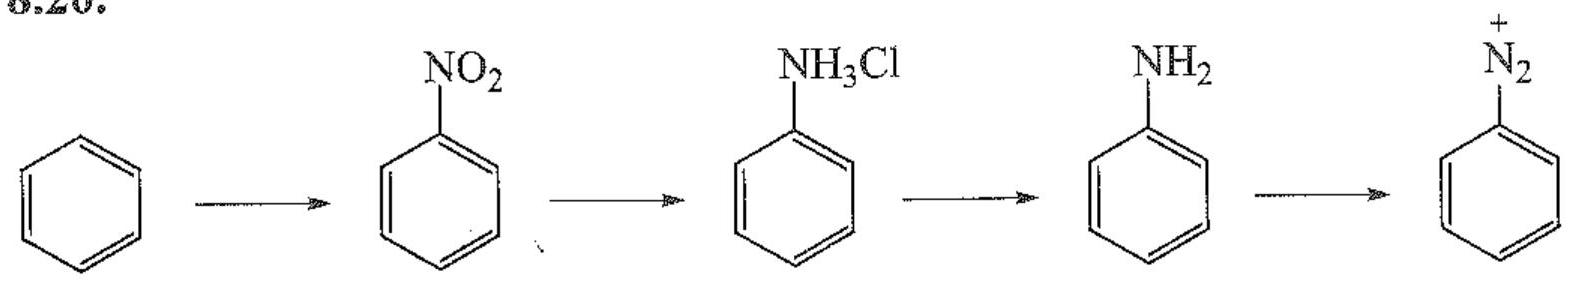
\includegraphics[max width=\textwidth, center]{2025_10_23_b82d44049ffb48e891e8g-11}\\
benzene\\
nitrobenzene phenylammonium chloride aniline $\_\_\_\_$ benzenediazonium\\
8.21. Trimethylamine là chất khí ở điều kiện thường, có tính base. Để khử mùi trimethylamine có thể sử dụng các loại acid hữu cơ có trong thực phẩm để chuyển trimethylamine thành muối tan không bay hơi. Các thực phẩm chứa acid hữu cơ có thể là giấm (chứa acetic acid), chanh (chứa citric acid), dứa (chứa citric acid, malic acid, ascorbic acid), me (tartaric acid, citric acid, malic acid, ascorbic acid),...\\
8.22. Amine làm nguyên liệu tổng hợp phẩm nhuộm Indigo Dye, polymer Polyurethane và dược phẩm Paracatamol là aniline. Amine làm nguyên liệu tổng hợp nylon-6,6 là hexamethylene diamine.\\
8.23. Adrenaline có chứa một nhóm amine bậc hai, một nhóm alcohol bậc hai và hai nhóm phenol; dopamine chứa hai nhóm phenol và một nhóm amine bậc một.\\
8.24. Phương pháp (1) có ưu điểm là điều chế được cả amine bậc một, bậc hai và bậc ba nhưng nhược điểm là không thu được sản phẩm tinh khiết mà là hỗn hợp các amine khác bậc.\\
Phương pháp (2) có ưu điểm tạo duy nhất amine bậc một nhưng nhược điểm là không điều chế được amine bậc hai và ba.

\section*{BAI 9. AMINO ACID VÀ PEPTIDE}
9.1. C\\
9.2. B\\
9.3. B\\
9.4. A\\
9.5. C\\
9.6. A\\
9.7. C\\
9.8. C\\
9.9. A\\
9.10. B\\
9.11. a) - đúng; b) - sai; c) - đúng; d) - đúng.\\
9.12. a) - đúng; b) - đúng; c) - đúng; d) - sai.\\
9.13. a) - sai; b) - đúng; c) - đúng; d) - đúng.\\
9.14. a) - sai; b) - sai; c) - đúng; d) - đúng.\\
9.15. a) - đúng; b) - đúng; c) - đúng; d) - đúng.\\
9.16. Có bốn dipeptide khác nhau gồm Gly-Gly, Ala-Ala, Gly-Ala và Ala-Gly.\\
9.17. Amino acid có nhiệt độ nóng chảy cao (đều là chất rắn ở điều kiện thường) và tan tốt trong nước do amino acid tồn tại chủ yếu dưới dạng ion lưỡng cực phân cực mạnh.\\
9.18. Amino acid có tính lưỡng tính do chứa đồng thời nhóm amino có tính base và nhóm carboxyl có tính acid.\\
Phương trình hoá học:\\
$\mathrm{HCl}+\mathrm{H}_{2} \mathrm{NCH}_{2} \mathrm{COOH} \longrightarrow \mathrm{ClH}_{3} \mathrm{NCH}_{2} \mathrm{COOH}$\\
$\mathrm{H}_{2} \mathrm{NCH}_{2} \mathrm{COOH}+\mathrm{NaOH} \longrightarrow \mathrm{H}_{2} \mathrm{NCH}_{2} \mathrm{COONa}+\mathrm{H}_{2} \mathrm{O}$\\
9.19. Nhúng quỳ tím vào mỗi mẫu thử, mẫu thử không đổi màu quỳ tím là dung dịch glycine; mẫu thử đổi màu quỳ tím sang màu xanh là dung dịch lysine và mẫu thử đổi màu quỳ tím sang màu đỏ là dung dịch glutamic acid.\\
9.20. Các amino acid thiên nhiên hầu hết là $\alpha$-amino acid (công thức chung có dạng $\left.\mathrm{H}_{2} \mathrm{~N}-\mathrm{CH}(\mathrm{R})-\mathrm{COOH}\right)$. Trong đó, chỉ có khoảng 20 amino acid cấu thành nên phần lớn protein trong cơ thể người, gọi là những amino acid tiêu chuẩn. Một số amino acid tiêu chuẩn mà cơ thể người không thể tự tổng hợp được, gọi là amino acid thiết yếu. Con người tiếp nhận amino acid thiết yếu qua thức ăn như thịt, cá, trứng, sữa,...\\
9.21. $\mathrm{H}_{3} \mathrm{~N}^{+} \mathrm{CH}_{2} \mathrm{COO}^{-} ; \mathrm{H}_{3} \mathrm{~N}^{+} \mathrm{CH}\left(\mathrm{CH}_{3}\right) \mathrm{COO}^{-} ; \mathrm{H}_{3} \mathrm{~N}^{+} \mathrm{CH}(i-\mathrm{Pr}) \mathrm{COO}^{-}$; $\mathrm{H}_{3} \mathrm{~N}^{+}-\left[\mathrm{CH}_{2}\right]_{4}-\mathrm{CH}\left(\mathrm{NH}_{2}\right) \mathrm{COO}^{-} ; \mathrm{HOOC}-\left[\mathrm{CH}_{2}\right]_{2}-\mathrm{CH}\left({ }^{+} \mathrm{NH}_{3}\right) \mathrm{COO}^{-}$.\\
9.22. Có thể sắp xếp các phân mảnh như sau (đảm bảo Ala là amino acid đầu C): Ala-His-Ser ... Ser-Asp-Phe ... Phe-Ala.\\
Từ đó, ta có đoạn mạch của F là Ala-His-Ser-Asp-Phe-Ala. Cấu tử cuối cùng của F phải là Phe trước Ala. Vậy, cấu tạo của F là Phe-Ala-His-Ser-Asp-Phe-Ala.\\
9.23. Kết hợp với các mảnh sinh ra do sự thuỷ phân không hoàn toàn Tyr-Gly và Gly-Gly-Phe (bỏ bớt một Gly do A chỉ là pentapeptit) ta có được trật tự liên kết giữa các amino acid là Tyr-Gly-Gly-Phe. Như vậy, Leu phải là amino acid đầu C, trật tự liên kết của các amino acid trong A là Tyr-Gly-Gly-Phe-Leu.\\
9.24. Xếp các phân mạnh theo nguyên tắc amino acid ở cuối mảnh này giống với amino acid ở đầu mảnh kế tiếp ta được:

Arg-Pro... Pro-Pro-Gly... Pro-Gly-Phe... Phe-Ser.. Ser-Pro-Phe... Arg\\
Lược bỏ các amino acid trùng lặp, ta có trật tự liên kết của các amino acid trong B là: Arg-Pro-Pro-Gly-Phe-Ser-Pro-Phe-Arg.

\section*{BAI 10. PROTEIN VÀ ENZYME}
10.1. A\\
10.2. B\\
10.3. D\\
10.4. a) - sai; b) - đúng; c) - đúng; d) - đúng.\\
10.5. a) - đúng; b) - đúng; c) - đúng; d) - đúng.\\
10.6. 2 .\\
10.7. 4.\\
10.8. 5.\\
10.9. Amylase và maltase đều đóng vai trò trong việc chuyển hoá thức ăn thành các chất dinh dưỡng cần thiết cho hoạt động sống của cơ thể, đảm bảo sức khoẻ cho con người. Ví dụ như amylase xúc tác cho quá trình thuỷ phân tinh bột, còn maltase xúc tác cho quá trình thuỷ phân maltose, đều tạo sản phẩm chính là glucose.\\
10.10. Một số người không thể tiêu hoá sữa do mắc chứng không dung nạp lactose (một loại đường có trong sữa). Nguyên nhân chính là do sự thiếu hụt enzyme lactase - một loại enzyme được sản xuất trong ruột non của người. Khi con người ăn hay uống các sản phẩm từ sữa mà không thể tiêu hoá hoàn toàn lactose, hậu quả là họ bị tiêu chảy và đầy hơi sau khi ăn hoặc uống các sản phẩm từ sữa.\\
10.11. Sự đa dạng trong thịt, cá, trứng và sữa cung cấp cho cơ thể đầy đủ những nguồn protein, khoáng chất và vitamin. Điều này giúp xây dựng và duy trì cơ bắp, hỗ trợ sự phát triển, củng cố hệ thống miễn dịch và duy trì sức khoẻ. Mỗi nguồn thực phẩm đều cung cấp một hỗn hợp riêng biệt của chất dinh dưỡng, giúp đảm bảo cơ thể nhận được đầy đủ các yếu tố cần thiết cho sự phát triển và hoạt động hằng ngày.\\
10.12.

\begin{enumerate}
  \item $\left(\mathrm{C}_{6} \mathrm{H}_{10} \mathrm{O}_{5}\right)_{\mathrm{n}}+\mathrm{nH}_{2} \mathrm{O} \xrightarrow{\text { Amylase }} \mathrm{nC}_{6} \mathrm{H}_{12} \mathrm{O}_{6}$
  \item $\mathrm{C}_{12} \mathrm{H}_{22} \mathrm{O}_{11}+\mathrm{H}_{2} \mathrm{O} \xrightarrow{\text { Maltase }} 2 \mathrm{C}_{6} \mathrm{H}_{12} \mathrm{O}_{6}$
  \item $\mathrm{C}_{6} \mathrm{H}_{12} \mathrm{O}_{6} \xrightarrow{\text { Enzyme }} 2 \mathrm{C}_{2} \mathrm{H}_{5} \mathrm{OH}+2 \mathrm{CO}_{2}$
  \item $\mathrm{C}_{2} \mathrm{H}_{5} \mathrm{OH}+\mathrm{O}_{2} \xrightarrow{\text { Enzyme }} \mathrm{CH}_{3} \mathrm{COOH}+\mathrm{H}_{2} \mathrm{O}$
\end{enumerate}

\section*{BAl 11 ÔN TẠP CHƯƠNG III}
\begin{center}
\begin{tabular}{lllll}
11.1. C & 11.2. A & 11.3. A & 11.4. C & 11.5. B \\
11.6. C & 11.7. B & 11.8. D & 11.9. C & 11.10. C \\
11.11. B & 11.12. D & 11.13. D & 11.14. A & 11.15. C \\
\end{tabular}
\end{center}

11.16. a) - đúng; b) - đúng; c) - đúng; d) - sai.\\
11.17. a) - sai; b) - sai; c) - dúng; d) - dúng.\\
11.18. a) - sai; b) - đúng; c) - sai; d) - đúng.\\
11.19. Phương trình hoá học:\\
$\mathrm{C}_{6} \mathrm{H}_{6}+\mathrm{HNO}_{3} \xrightarrow{\mathrm{H}_{2} \mathrm{SO}_{4}} \mathrm{C}_{6} \mathrm{H}_{5} \mathrm{NO}_{2}+\mathrm{H}_{2} \mathrm{O}$\\
$\mathrm{C}_{6} \mathrm{H}_{5} \mathrm{NO}_{2}+6[\mathrm{H}] \xrightarrow{\mathrm{Fe} / \mathrm{HCl}} \mathrm{C}_{6} \mathrm{H}_{5} \mathrm{NH}_{2}+2 \mathrm{H}_{2} \mathrm{O}$\\
11.20. Aniline có tính base rất yếu do nhóm phenyl hứt electron làm giảm mật độ electron trên nguyên tử nitrogen và nguyên tử nitrogen này khó nhường cặp electron.\\
11.21. (1) Glycine có một nhóm amine ( $-\mathrm{NH}_{2}$ ) và một nhóm carboxyl ( -COOH ), môi trường gần trung tính nên không làm đổi màu quỳ tím.\\
(2) Lysine có hai nhóm amine ( $-\mathrm{NH}_{2}$ ) và một nhóm carboxyl ( -COOH ), phản ứng với nước tạo môi trường kiềm nên làm đồi màu quỳ tím sang màu xanh.\\
$\mathrm{H}_{2} \mathrm{~N}\left[\mathrm{CH}_{2}\right]_{4} \mathrm{CH}\left(\mathrm{NH}_{2}\right) \mathrm{COOH}+\mathrm{H}_{2} \mathrm{O} \rightleftharpoons \mathrm{H}_{3} \mathrm{~N}^{+}\left[\mathrm{CH}_{2}\right]_{4} \mathrm{CH}\left({ }^{+} \mathrm{NH}_{3}\right) \mathrm{COO}^{-}+\mathrm{OH}^{-}$\\
(3) Glutamic acid có một nhóm amine ( $-\mathrm{NH}_{2}$ ) và hai nhóm carboxyl ( -COOH ), phản ứng với nước tạo môi trường acid nên làm đổi màu quỳ tím sang màu đỏ.\\
$\mathrm{HOOC}\left[\mathrm{CH}_{2}\right]_{2} \mathrm{CH}\left(\mathrm{NH}_{2}\right) \mathrm{COOH}+\mathrm{H}_{2} \mathrm{O} \rightleftharpoons-\mathrm{OOC}\left[\mathrm{CH}_{2}\right]_{2} \mathrm{CH}\left({ }^{+} \mathrm{NH}_{3}\right) \mathrm{COO}^{-}+\mathrm{H}_{3} \mathrm{O}^{+}$

\section*{Churong IV POLYMER}
\section*{BAI 12 ĐAI CƯONG VỂ POLYMER.}
12.1. D 12.2. D 12.3. B\\
12.4. D 12.5. C 12.6. C\\
12.7. B 12.8.A : 12.9.A\\
12.10. D 12.13. A\\
12.11. a) - đúng; b) - sai; c) - đúng; d) - đúng.\\
12.12. Polystyrene có công thức cấu tạo là:

$$
\begin{aligned}
&+\mathrm{CH}_{2}-\mathrm{CH}\left(\mathrm{C}_{6} \mathrm{H}_{5}\right)_{\mathrm{n}} \\
& \Rightarrow 104 \mathrm{n}=264160 \Rightarrow \mathrm{n}=2540
\end{aligned}
$$

12.14. a) - sai; b) - đúng; c) - đúng; d) - đúng.\\
12.15. Phương trình họá học:\\
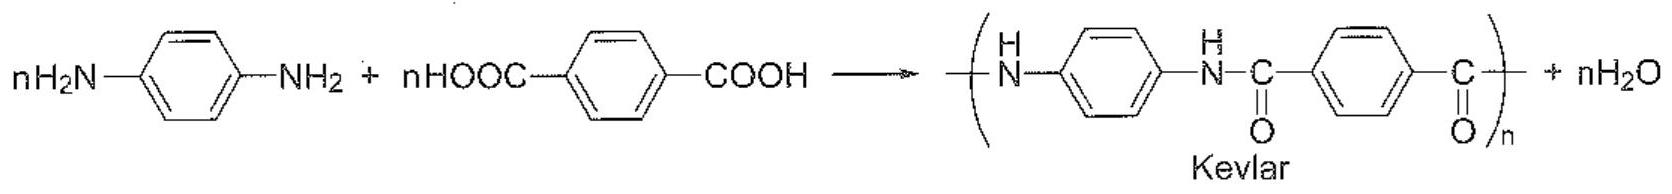
\includegraphics[max width=\textwidth, center]{2025_10_23_b82d44049ffb48e891e8g-15}

Phản ứng tổng hợp Kevlar thuộc loại phản úng trùng ngưng.\\
12.16. a) Phương trình hoá học:\\
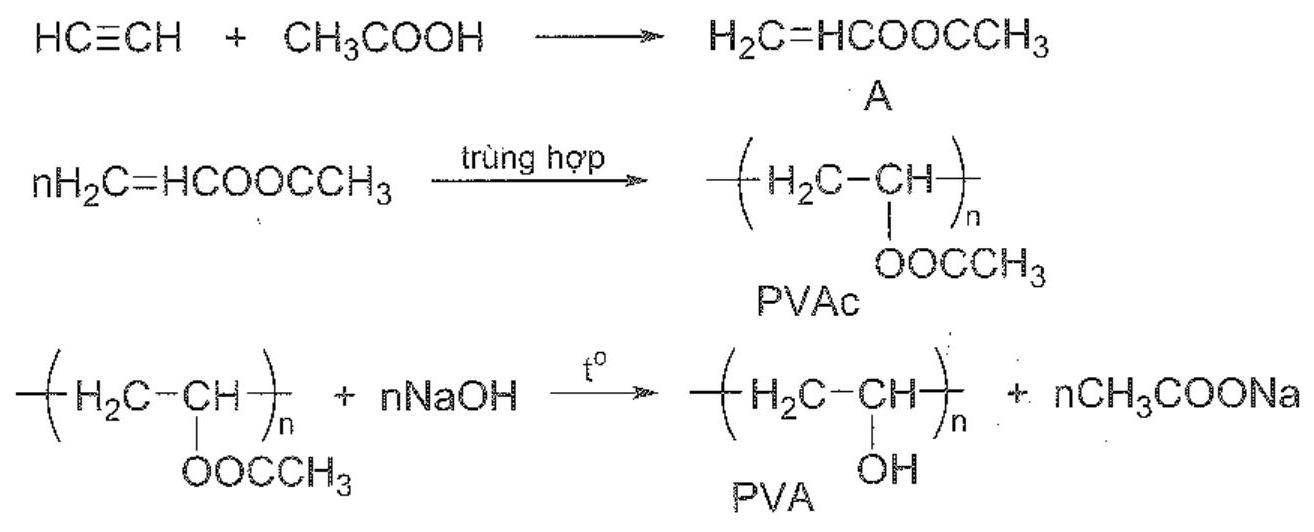
\includegraphics[max width=\textwidth, center]{2025_10_23_b82d44049ffb48e891e8g-15(1)}\\
b) Do PVA có chưa các nhóm chức alcohol, có khả năng tạo liên kết hydrogen với nước nêm tan đực trong nước.

\section*{BAI 13 VÂT LIỆU POLYMER}
\begin{center}
\begin{tabular}{lllll}
13.1. D & 13.2. C & 13.3. A & 13.4. A & 13.5. B \\
13.6. A & 13.7. A & 13.8. C & 13.9. D & 13.10. D \\
13.11. A & 13.14. B &  &  &  \\
\end{tabular}
\end{center}

13.12. a) - đúng; b) - sai; c) - sai; d) - đúng.\\
13.13. Vật liệu cốt: bột gỗ.

Vật liệu nền: nhựa polyethylene.\\
13.15. a) - đúng; b) - sai; c) - đúng; d) - sai.\\
13.16. a) - đúng; b) - sai, c) - sai; d) - đúng.\\
13.17\%\\
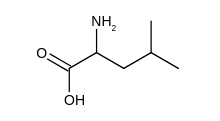
\includegraphics{smile-7933d0a12d1d333811a6a56bfe4cc3114d5b40f1}\\
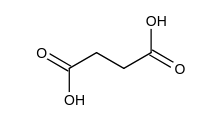
\includegraphics{smile-d6029b54401fe1ae02b4808b9aaaa5d37509bde0}\\
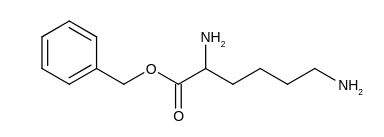
\includegraphics{smile-8d79f9024eb8bddc2281ded4eaf64bd3383fba75}\\
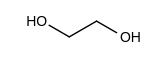
\includegraphics{smile-25a774e1892adb46bee7e04bbc5c470218b309a5}

\section*{BAI 14 ÔN TÂP CHUONG IV}
14.1. D\\
14.2. A\\
14.3. A\\
14.4. C\\
14.5. D\\
14.6. A\\
14.7. B\\
14.8. A\\
14.9. D\\
14.10. a) - sai; b) - đúng; c) - đúng; d) - đúng.\\
14.11. a) - sai; b) - đúng; c) - sai; d) - đúng.\\
14.12. Trong tơ tằm và tơ polyamide có các liên kết - $\mathrm{CO}-\mathrm{NH}-$, các liên kết này không bền, dễ bị thuỷ phân trong môi trường kiềm nên làm giảm độ bền của quần áo.\\
14.13. a) Phương trình hoá học:\\
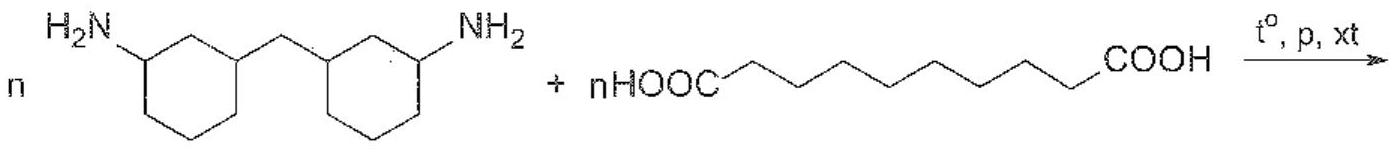
\includegraphics[max width=\textwidth, center]{2025_10_23_b82d44049ffb48e891e8g-16}\\
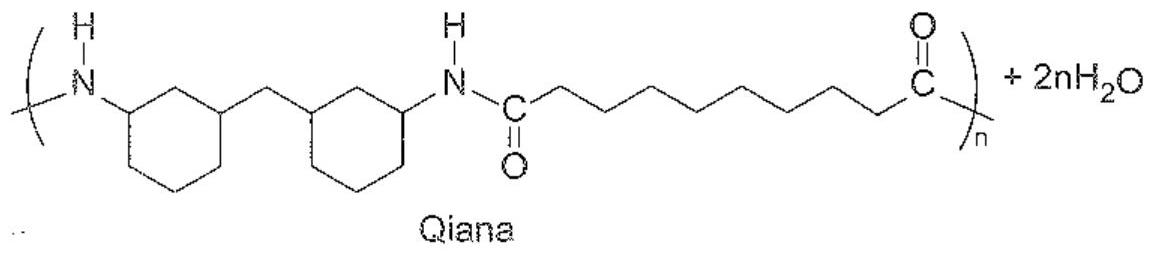
\includegraphics[max width=\textwidth, center]{2025_10_23_b82d44049ffb48e891e8g-16(1)}

Phản ứng tổng hợp Qiana thuộc loại phản ứng trùng ngung.\\
b) Tơ Qiana thuộc loại tơ tổng hợp (polyamide). Tơ này kém bền trong môi trường acid hoặc base mạnh do dễ bị thuỷ phân.\\
14.14. a) Nhựa PET được điều chế bằng phản ứng trùng ngưng terephthalic acid với ethylene glycol:\\
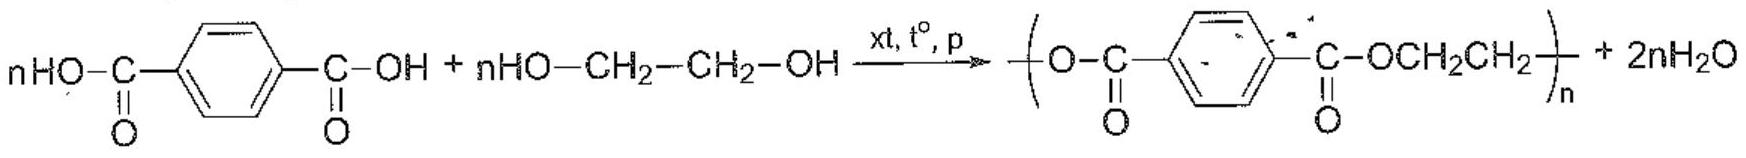
\includegraphics[max width=\textwidth, center]{2025_10_23_b82d44049ffb48e891e8g-17(2)}\\
b) Theo kí hiệu nhận dạng thì nhựa PET có thể tái chế được và thuộc loại nhựa nhiệt đẻo.\\
c) Phưong trình hoá học:\\
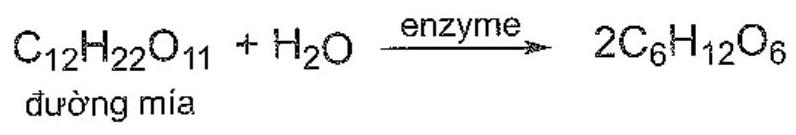
\includegraphics[max width=\textwidth, center]{2025_10_23_b82d44049ffb48e891e8g-17}\\
$\mathrm{C}_{6} \mathrm{H}_{12} \mathrm{O}_{6} \xrightarrow{\text { enzyme }} 2 \mathrm{C}_{2} \mathrm{H}_{5} \mathrm{OH}+2 \mathrm{CO}_{2}$\\
$\mathrm{C}_{2} \mathrm{H}_{5} \mathrm{OH} \xrightarrow{\mathrm{xt}_{,} \mathrm{t}^{\circ}} \mathrm{CH}_{2}=\mathrm{CH}_{2}+\mathrm{H}_{2} \mathrm{O}$\\
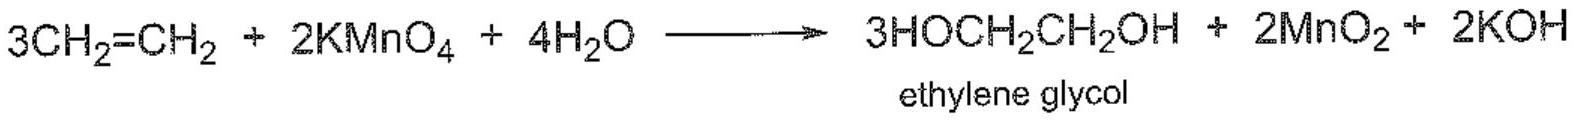
\includegraphics[max width=\textwidth, center]{2025_10_23_b82d44049ffb48e891e8g-17(1)}

\section*{Chưong V PIN DIEN VA DIEN PHAN}
\section*{BÀ 15. THẾ ĐIỆN CỰC VÀ NGUỒN ĐIỆN HOÁ HỌC}
\begin{center}
\begin{tabular}{|l|l|l|l|l|}
\hline
15.1. B & 15.2.A & 15.3. B & 15.4.D & 15.5. C \\
\hline
15.6. D & 15.7.A & 15.8. D & 15.9. C & 15.10. C \\
\hline
15.11. A & 15.12.A & 15.13. A & 15.14. C & 15.15. B \\
\hline
15.16. A & 15.17. D & 15.18. D & 15.19. C & 15.20. A \\
\hline
15.21. B & 15.22. D & 15.23. D & 15.24. B & 15.25. A \\
\hline
15.26. A & 15.32. D & 15.33. A & 15.34.A &  \\
\hline
\end{tabular}
\end{center}

15.27. a) - đúng; b) - đúng; c) - đúng; d) - sai.\\
15.28. a) - đúng; b) - sai; c) - đúng; d) - sai.\\
15.29. a) - sai; b) - đúng; c) - đúng; d) - đúng.\\
15.30. 0,48.\\
15.31. 1,24.\\
15.35. a) - đúng; b) - đúng; c) - sai; d) - sai.\\
15.36. a) - đúng; b) - sai; c) - đúng; d) đúng.\\
15.37. 0,51.\\
15.38. 0,40.

\section*{BAl 16 ĐIỆN PHÂN}
\begin{center}
\begin{tabular}{lll}
16.1. B & 16.2. C & 16.3. A \\
16.4. D & 16.5. A & 16.6. C \\
16.7. B & 16.8. A & 16.9. D \\
16.10. B & 16.11. A & 16.12. D \\
16.13. C & 16.14. B & 16.15. A \\
16.16. A & 16.17. B & 16.18. B \\
16.19. D & 16.20. B & 16.21. B \\
16.22. B & 16.23. B & 16.24. C \\
16.30. C & 16.31. C &  \\
\end{tabular}
\end{center}

16.25. a) - sai; b) - sai; c) - sai; d) - đúng.\\
16.26. a) - đúng; b) - sai; c) - đúng; d) - sai.\\
16.27. a) - đúng; b) - đúng; c) - sai; d) - đúng.\\
16.28. Số mol electron: $\mathrm{n}_{\mathrm{e}}=1 \cdot \mathrm{n}_{\mathrm{Ag}}=0,0463 \mathrm{~mol}$.

Điện lượng $\mathrm{q}=\mathrm{n}_{\mathrm{e}} \cdot \mathrm{F}=4468 \mathrm{C}$\\
$\Rightarrow \mathrm{t}=\frac{\mathrm{q}}{\mathrm{I}}=\frac{4468 \mathrm{C}}{1,5 \mathrm{~A}}=2978 \mathrm{~s}=49,6 \mathrm{~min}$.\\
16.29. Quá trình oxi hoá ở anode: $\mathrm{Cu} \rightarrow \mathrm{Cu}^{2+}+2 \mathrm{e}$

Số mol electron: $\mathrm{n}_{\mathrm{e}}=2 \cdot \mathrm{n}_{\mathrm{Cu}}=3,125 \mathrm{~mol}$.\\
Điện lượng $\mathrm{q}=\mathrm{n}_{\mathrm{e}} \cdot \mathrm{F}=301563 \mathrm{C} \Rightarrow \mathrm{t}=\frac{\mathrm{q}}{\mathrm{I}}=\frac{301563 \mathrm{C}}{28800 \mathrm{~s}}=2978 \mathrm{~s}=10,5 \mathrm{~A}$.\\
16.32. a) đúng; b) đúng: c) đúng; d) sai.\\
16.33. 0,60.\\
16.34, 1,25.\\
16.35. 3860.\\
16.36. 0,03 .

\section*{BAI 17. ÔN TẬP CHƯƠNG V}
17.1. B\\
17.2. D\\
17.3. D\\
17.4. A\\
17.5. D\\
17.6. C\\
17.7. D\\
17.8. C\\
17.9. B\\
17.10. B\\
17.11. C\\
17.12. a) - sai; b) - đúng; c) - đúng; d) - đúng.\\
17.13. a) - đúng; b) - sai: c) - đúng; d) - sai.\\
17.14. a) - đúng; b) - đúng; c) - sai; d) - đúng.\\
17.15. 0,90.\\
17.16, 0,77.\\
17.17. 11,3.

\section*{Chưong VI \\
 DAI CUONG VER KIM LOAI}
\section*{BÀ 18. CẤU TAO VÀ LIÊN KẾT TRONG TINH THỂ KIM LOAI}
18.1. C 18.2. C\\
18.3. A 18.4. B\\
18.5. A 18.6. A\\
18.7. A 18.8. D\\
18.9. a) - đúng; b) - đúng; c) - sai; d) - đúng.\\
18.10. a) - đúng; b) - đúng; c) - sai; d) - đúng.\\
18.11. a) - đúng; b) - đúng; c) - đúng; d) - đúng.

\section*{BÀl 19 TÍNH CHẤT VẬT LÍ VÀ TÍNH CHẤT HOÁ HOC CỦA KIM LOẠI}
19.1. D 19.2. A\\
19.3. D 19.4. D\\
19.5. D 19.6. A\\
19.10. B 19.11. A\\
19.12. A 19.13. A\\
19.17. A 19.18. B\\
19.7. a) - đúng; b) - sai; c) - sai; d) - đúng.\\
19.8. a) - đúng; b) - đúng; c) - sai; d) - đúng.\\
19.9. (1) không; (2) không; (3) có; (4) có.\\
19.14. 1,92.\\
19.15. 0,07.\\
19.16. 31,7.\\
19.19. 0,24.\\
19.20. 800.\\
19.21. 0,3.

\section*{BAI 20. KIM LOAI TRONG TỰ NHIÊN VÀ PHƯƠNG PHÁP TÁCH KIM LOAI}
20.1. B 20.2. C\\
20.3. A 20.4. B\\
20.5. C 20.6. B\\
20.7. D 20.8. D\\
20.9. A 20.10. C\\
20.11. C 20.12. C\\
20.13. A 20.16. B\\
20.14. a) - sai; b) - đúng; c) - đúng; d) - sai.\\
20.15. 11,2.\\
20.17. a) - sai; b) - đúng; c) - đúng; d) - sai\\
20.18. a) - đúng; b) - đúng; c) - đúng; d) - đúng.

\section*{BAI 21 HƠP KIM}
\begin{center}
\begin{tabular}{lll}
21.1. C & 21.2. C & 21.3. D \\
21.4. B & 21.5. A & 21.6. A \\
21.8. C & 21.9. A & 21.10. C \\
21.11. C & 21.12. A & 21.13. A \\
21.14. C &  &  \\
\end{tabular}
\end{center}

21.7. a) - đúng; b) - sai; c) - sai; d) - sai.

\section*{BAll22 SỰĂN MÒN KIM LOAI}
22.1.C 22.2.A\\
22.3. A 22.4. B\\
22.5. D 22.6. B\\
22.7.C 22.8.C\\
22.9.A 22.10.A\\
22.11. B 22.12. C\\
22.13. D: 22.14. B\\
22.15. D\\
22.16. 191.\\
22.17. a) - sai; b) - đúng; c) - sai; d) - sai.\\
22.18. a) - sai; b) - đúng; c) - sai; d) - đúng.

\section*{BAl 23. ÔN TẬP CHƯƠNG VI}
23.1. A 23.2. B\\
23.3. C 23.4. B\\
23.5. A 23.6. D\\
23.7. B 23.8. D\\
23.9. B 23.10. A\\
23.11. A 23.12. B\\
23.13. C\\
23.14. a) - sai; b) - đúng; c) - sai; d) - đúng.\\
23.15. 32.\\
23.16. 0,5.\\
23.17.70,2.\\
23.18. 88,2.

\section*{Chưong VII NGUYÊN TO NHÓM IA VÀ NHÓM IIA}
\section*{BAI 24 NGUYÊN TỐ NHÓM IA}
\begin{center}
\begin{tabular}{|l|l|l|}
\hline
24.1. B & 24.2. D & 24.3. A \\
\hline
24.4. D & 24.5. C & 24.6. B \\
\hline
24.7. C & 24.8. C & 24.9. A \\
\hline
24.10. C & 24.11.B & 24.12. D \\
\hline
24.13. A & 24.14. A & 24.15. C \\
\hline
24.16. D & 24.17. A & 24.18. A \\
\hline
24.19. C & 24.20. B & 24.21. A \\
\hline
24.22. A & 24.23. D & 24.24. B \\
\hline
24.25. A & 24.26. B & 24.27. A \\
\hline
24.28. A & 24.29. D & 24.30. C \\
\hline
24.36. C & 24.37. B & 24.38. A \\
\hline
\end{tabular}
\end{center}

24.31. a) - đúng; b) - sai; c) - sai; d) - đúng.\\
24.32. a) - sai; b) - đúng; c) - sai; d) - đúng.\\
24.33. Nồng độ phần trăm:

$$
C=\frac{S}{100+S} \cdot 100 \%=\frac{35,9}{100+35,9} \cdot 100 \%=26,4 \% .
$$

24.34. Tổng bán kính ion $\mathrm{Na}^{+}$và ion $\mathrm{Cl}^{-}=\frac{\mathrm{a}}{2}=\frac{564 \mathrm{pm}}{2}=282 \mathrm{pm}$.\\
$\Rightarrow$ Bán kính ion $\mathrm{Na}^{+}=100 \mathrm{pm}$.\\
24.35. Số mol NaOH tối thiểu cần dùng: $\frac{1000000}{102} \cdot 2=19608(\mathrm{~mol})$.

Khối lượng dung dịch: $40 \cdot 19608 \cdot \frac{100}{20}=3921600(\mathrm{~g})=3,9216$ tấn.\\
24.39. a) - đúng; b) - sai; c) - sai; d) - sai.\\
24.40. a) - sai; b) - đúng; c) - đúng; d) - đúng.\\
24.41. 0,1.\\
24.42. 1,4.

\section*{BAI 25. NGUYÊN TỐ NHÓM IIA}
25.1. B 25.2.A 25.3.C\\
25.4.C 25.5.D 25.6.A\\
25.7. B 25.8. B 25.9. C\\
25.10.C 25.11.D 25.12.A\\
25.13. B 25.14. D 25.15. A\\
25.16. D 25.17. D 25.18. C\\
25.19. C 25.20. B 25.21. A\\
25.22. C 25.23. D 25.24. C\\
25.25. C 25.26. C 25.27. A\\
25.28. B 25.29. D 25.30. D\\
25.31. B 25.32. D 25.33. A\\
25.34. D\\
25.35. a) - đúng; b) - sai; c) - đúng; d) - sai.\\
25.36. a) - sai; b) - đúng; c) - sai; d) - đúng.\\
25.37. a) - đúng; b) - sai; c) - đúng; d) - đúng.\\
25.38. Độ tan trong nước của $\mathrm{Ca}(\mathrm{OH})_{2}$ là $1,73 \mathrm{~g}$ trong 1 lít nước.

Nồng độ mol của nước vôi trong bão hoà:

$$
C_{M}=\frac{1,73}{1 \cdot 74}=0,0234(M)=2,34 \cdot 10^{-2} M
$$

25.39. Biến thiên enthalpy chuẩn của phản ứng:

$$
\Delta_{\mathrm{r}} \mathrm{H}_{298}^{\mathrm{o}}=-601,6+33,1 \cdot 2-(-790,6)=255,2(\mathrm{~kJ}) .
$$

25.40. Trong $1 \mathrm{~cm}^{3}$ tinh thể kim loại Ca thì các quả cầu kim loại chiếm thể tích $0,74 \mathrm{~cm}^{3}$ và có khối lượng $1,55 \mathrm{~g}$.

Số quả cầu kim loại $=6,023 \cdot 10^{23} \cdot \frac{1,55}{40}=0,2334 \cdot 10^{23}=0,02334 \cdot 10^{24}$.\\
Tô̂ng thể tích các quả cầu kim loại:\\
$\frac{4}{3} \cdot \pi \cdot \mathrm{r}^{3} \cdot 0,02334 \cdot 10^{24}=0,74\left(\mathrm{~cm}^{3}\right) \Rightarrow \mathrm{r}=1,96 \cdot 10^{-8} \mathrm{~cm}=196 \mathrm{pm}$.\\
25.41. 80.

\section*{BAI 26. ÔN TẬP CHƯƠNG VII}
\begin{center}
\begin{tabular}{lll}
26.1. C & $26.2 . \mathrm{D}$ & $26.3 . \mathrm{A}$ \\
$26.5 . \mathrm{B}$ & $26.6 . \mathrm{C}$ & $26.7 . \mathrm{A}$ \\
$26.8 . \mathrm{C}$ & $26.9 . \mathrm{D}$ & $26.10 . \mathrm{A}$ \\
$26.11 . \mathrm{B}$ & $26.12 . \mathrm{D}$ & $26.13 . \mathrm{C}$ \\
$26.14 . \mathrm{A}$ & $26.15 . \mathrm{A}$ & $26.16 . \mathrm{A}$ \\
$26.17 . \mathrm{A}$ & $26.18 . \mathrm{B}$ & $26.19 . \mathrm{A}$ \\
\end{tabular}
\end{center}

26.20. a) - đúng; b) - đúng; c) - sai; d) - sai.\\
26.21. a) - sai; b) - đúńg; c) - đúng; d) - sai.\\
26.22. Số $\mathrm{mol} \mathrm{CO}_{2}=\frac{1,408}{44}=0,032$ (mol);

Số $\mathrm{mol} \mathrm{BaCO}_{3}=\frac{3,152}{197}=0,016(\mathrm{~mol})$.\\
Bảo toàn nguyên tố C : Số $\mathrm{mol} \mathrm{CO}_{2}=$ Số $\mathrm{mol} \mathrm{BaCO}_{3}+$ Số $\mathrm{mol} \mathrm{Ba}\left(\mathrm{HCO}_{3}\right)_{2} \cdot 2$\\
$\Rightarrow$ Số $\mathrm{mol} \mathrm{Ba}\left(\mathrm{HCO}_{3}\right)_{2}=0,008 \mathrm{~mol}$.\\
Bảo toàn nguyên tố Ba :\\
Số $\mathrm{mol} \mathrm{Ba}(\mathrm{OH})_{2}=$ Số $\mathrm{mol} \mathrm{BaCO}_{3}$ + Số $\mathrm{mol} \mathrm{Ba}\left(\mathrm{HCO}_{3}\right)_{2}=0,024 \mathrm{~mol}$\\
$\Rightarrow \mathrm{a}=\frac{0,024}{0,3}=0,08$.\\
26.23. Số tiền mua vôi $=20$ nghìn đồng $\frac{2 \cdot 720}{100}=288$ nghìn đồng.\\
26.24. 0,05 .\\
26.25. 4,8.

\section*{Chưong VIII \\
 SO LƯỢC VỂ DÁY KIM LOAI CHUYÊN TIÉP THƯ NHÁT VA PHÚC CHÁT}
\section*{BAI 27 ĐAI CUƠNG VÊ̂ KIM LOAI CHUYỂN TIẾP DÃY THỨ NHẤT}
27.1. A 27.2. C 27.3. C\\
27.4. A 27.5. D 27.6. A\\
27.7. B 27.8. D 27.9. D\\
27.10. C 27.11. C 27.12. A\\
27.13. B 27.14. A 27.15. C\\
27.16. C 27.17. D 27.18. B\\
27.19. B 27.20.A 27.21.D\\
27.22. C 27.23. A 27.24. B\\
27.25. D 27.26. A 27.27. B\\
27.28. A 27.29. B 27.30. B\\
27.31. C 27.32. A 27.33. C\\
27.34. D 27.35. D 27.41. B\\
27.42. C 27.43. D 27.44. D\\
27.36. a) - đúng; b) - sai; c) - đúng; d) - sai.\\
27.37. a) - đúng; b) - sai; c) - đúng; d) - sai.\\
27.38. Phương trình hoá học của phản ứng:\\
$10 \mathrm{FeSO}_{4}+2 \mathrm{KMnO}_{4}+8 \mathrm{H}_{2} \mathrm{SO}_{4} \longrightarrow 5 \mathrm{Fe}_{2}\left(\mathrm{SO}_{4}\right)_{3}+\mathrm{K}_{2} \mathrm{SO}_{4}+2 \mathrm{MnSO}_{4}+8 \mathrm{H}_{2} \mathrm{O}$\\
Nồng độ mol của dung dịch $\mathrm{FeSO}_{4}$ ban đầu:

$$
\mathrm{a}=\frac{8,80 \cdot 0,02 \cdot 5}{10,00} \cdot 10=0,88 .
$$

27.39. Độ tan trong nước của $\mathrm{CuSO}_{4} \cdot 5 \mathrm{H}_{2} \mathrm{O}$ là 32 g trong 100 g nước.

Nồng độ phần trăm của $\mathrm{CuSO}_{4}$ :

$$
\frac{32}{132} \cdot \frac{160}{250} \cdot 100 \%=15,5 \%
$$

27.40. Trong $1 \mathrm{~cm}^{3}$ tinh thể kim loại Fe thì các quả cầu kịm loại chiếm thể tích $0,68 \mathrm{~cm}^{3}$ và có khối lượng $7,87 \mathrm{~g}$.\\
Số quả cầu kim loại $=6,023 \cdot 10^{23} \cdot \frac{7,87}{55,85}=0,8487 \cdot 10^{23}=0,08487 \cdot 10^{24}$.\\
Tổng thể tích các quả cầu kim loại:\\
$\frac{4}{3} \cdot \pi \cdot \mathrm{r}^{3} \cdot 0,08487 \cdot 10^{24}=0,68\left(\mathrm{~cm}^{3}\right) \Rightarrow \mathrm{r}=1,24 \cdot 10^{-8} \mathrm{~cm}=124 \mathrm{pm}$.\\
27.41. Xét cân bằng:

$$
\mathrm{Fe}^{3+}(\mathrm{aq})+\mathrm{H}_{2} \mathrm{O}(l) \rightleftharpoons[\mathrm{Fe}(\mathrm{OH})]^{2+}(\mathrm{aq})+\mathrm{H}^{+}(\mathrm{aq}) \quad \mathrm{K}_{\mathrm{a}}=10^{-2,19}
$$

[]: $0,1-\mathrm{x}$\\
x\\
x\\
$\mathrm{K}_{\mathrm{C}}=\frac{[\mathrm{Fe}(\mathrm{OH})]^{2+}\left[\mathrm{H}^{+}\right]}{\left[\mathrm{Fe}^{3+}\right]}=10^{-2,19} \Rightarrow \frac{\mathrm{x}^{2}}{0,1-\mathrm{x}}=10^{-2,19}$\\
$\Rightarrow \mathrm{x}=0,022 \mathrm{M} \Rightarrow\left[\mathrm{H}^{+}\right]=0,022 \mathrm{M} \Rightarrow \mathrm{pH}=-\lg 0,022=1,66$.\\
27.42.\\
$\mathrm{Cr}_{2} \mathrm{O}_{7}^{2-}+\mathrm{H}_{2} \mathrm{O} \rightleftharpoons 2 \mathrm{CrO}_{4}^{2-}+2 \mathrm{H}^{+}$

$$
\mathrm{K}_{\mathrm{C}}=10^{-15,2}
$$

$0,1-\mathrm{x}$

$$
2 \mathrm{x} \quad 10^{-6}
$$

$\mathrm{K}_{\mathrm{C}}=\frac{\left[\mathrm{CrO}_{4}^{2-}\right]^{2}\left[\mathrm{H}^{+}\right]^{2}}{\left.\mathrm{Cr}_{2} \mathrm{O}_{7}^{2-}\right]}=\frac{(2 \mathrm{x})^{2}\left(10^{-6}\right)^{2}}{0,1-\mathrm{x}}=10^{-15,2} \Rightarrow \mathrm{x}=3,9 \cdot 10^{-3}$.\\
Phần trăm $\mathrm{Cr}_{2} \mathrm{O}_{7}^{2-}$ đã chuyển hoá $=\frac{3,9 \cdot 10^{-3}}{0,1} \cdot 100 \%=3,9 \%$.\\
27.43. Dung dịch $\mathrm{FeCl}_{3}$ bão hoà ở $0^{\circ} \mathrm{C}$ :

$$
\mathrm{C} \%=\frac{162,5}{270,5} \cdot \frac{74,4}{100+74,4} \cdot 100 \%=25,6 \%
$$

27.44. Khối lượng $\mathrm{H}_{2} \mathrm{C}_{2} \mathrm{O}_{4} \cdot 2 \mathrm{H}_{2} \mathrm{O}$ cần dùng $=126,07 \cdot 0,005=0,630(\mathrm{~g})$.

Phương trình hoá học của phản ứng chuẩn độ:

$$
5 \mathrm{H}_{2} \mathrm{C}_{2} \mathrm{O}_{4}+2 \mathrm{KMnO}_{4}+3 \mathrm{H}_{2} \mathrm{SO}_{4} \xrightarrow{\mathrm{t}^{\circ}} 10 \mathrm{CO}_{2}+\mathrm{K}_{2} \mathrm{SO}_{4}+2 \mathrm{MnSO}_{4}+8 \mathrm{H}_{2} \mathrm{O}
$$

Nồng độ dung dịch $\mathrm{KMnO}_{4}$ :

$$
\frac{2}{5} \cdot \frac{5,00 \cdot 0,05}{5,10}=0,0196(\mathrm{M})=1,96 \cdot 10^{-2} \mathrm{M}
$$

27.45. a) - đúng.

Tinh thể Cr có liên kết kim loại mạnh hơn tinh thể K vì đều có cùng cấu trúc tinh thể nhưng lại có nhiệt độ nóng chảy và độ cứng cao hơn.\\
b) - sai.

Tinh thể Cr có khối lượng riêng lớn hơn tinh thể K nên có khối lượng kim loại nhiều hơn.\\
c) - sai.

Nguyên tử Cr và nguyên tử K đều có 4 lớp electron nhưng nguyên tử Cr có điện tích hạt nhân lớn hơn.\\
d) - đúng.

K là kim loại nhẹ $\left(\mathrm{D}<5 \mathrm{~g} / \mathrm{cm}^{3}\right)$ và Cr là kim loại nặng $\left(\mathrm{D}>5 \mathrm{~g} / \mathrm{cm}^{3}\right)$.\\
27.46. a) - đúng.

Độ dài đường chéo hình vuông bằng 4 lần bán kính:

$$
\begin{gathered}
d=a \sqrt{2}=4 r \\
\Rightarrow r=\frac{a \sqrt{2}}{4}=\frac{361 \mathrm{pm} \sqrt{2}}{4}=128 \mathrm{pm}
\end{gathered}
$$

b) - sai.

Trong mỗi hình lập phương, mỗi nguyên tử Cu ở đỉnh đóng góp $\frac{1}{8}$ thể tích, mỗi nguyên tử ở mặt đóng góp $\frac{1}{2}$ thể tích.\\
Tổng số nguyên tử $\mathrm{Cu}=\frac{1}{8} \cdot 8+\frac{1}{2} \cdot 6=4$ (nguyên tử).\\
c) - đúng.

Khối lượng riêng $=\frac{\text { Khối lượng các quả cầu kim loại }}{\text { Thể tích hình lập phương }}$

$$
\mathrm{D}=\frac{63,54 \cdot 4 \cdot 1,66 \cdot 10^{-24} \mathrm{~g}}{\left(3,61 \cdot 10^{-8} \mathrm{~cm}\right)^{3}}=\frac{63,54 \cdot 4 \cdot 1,66 \mathrm{~g}}{3,61^{3} \mathrm{~cm}^{3}}=8,97 \mathrm{~g} / \mathrm{cm}^{3}
$$

d) - đúng.

Hệ số chặt khít $=\frac{\text { Thể tích } 4 \text { quả cầu }}{\text { Thể tích ô cơ sở }}$\\
$\rho=\frac{4\left(\frac{4}{3}\right) \pi r^{3}}{a^{3}}=\frac{4\left(\frac{4}{3}\right) \pi\left(\frac{a \sqrt{2}}{4}\right)^{3}}{a^{3}}=\frac{\pi \sqrt{2}}{6} \approx 0,74=74 \%$.\\
27.47. $\mathrm{Fe}_{2}\left(\mathrm{SO}_{4}\right)_{3}+3 \mathrm{Ca}(\mathrm{OH})_{2} \longrightarrow 2 \mathrm{Fe}(\mathrm{OH})_{3}+3 \mathrm{CaSO}_{4}$


\begin{equation*}
4 \mathrm{FeSO}_{4}+4 \mathrm{Ca}(\mathrm{OH})_{2}+\mathrm{O}_{2}+2 \mathrm{H}_{2} \mathrm{O} \longrightarrow 4 \mathrm{Fe}(\mathrm{OH})_{3}+4 \mathrm{CaSO}_{4} \tag{1}
\end{equation*}


Khối lượng sắt có trong $10 \mathrm{~m}^{3}$ nước $=0,30 \cdot 28 \cdot 10000=84000(\mathrm{mg})=84(\mathrm{~g})$.\\
Số $\mathrm{mol} \mathrm{Fe}^{3+}$ và $\mathrm{Fe}^{2+}$ tương ứng là $0,3 \mathrm{~mol}$ và $1,2 \mathrm{~mol}$.\\
Tổng số $\mathrm{mol} \mathrm{OH}^{-}$cần dùng $=0,3 \cdot 3+1,2 \cdot 2=3,3(\mathrm{~mol})$.\\
$\Rightarrow$ Số $\mathrm{mol} \mathrm{Ca}(\mathrm{OH})_{2}=1,65 \mathrm{~mol}$\\
$\Rightarrow$ Khối lượng vôi tôi $=74 \cdot 1,65=122,1(\mathrm{~g}) \sim 122 \mathrm{~g}$.\\
27.48. Công thức của muối carbonate là $\mathrm{MCO}_{3}$.

$$
\frac{\% \mathrm{M}}{\% \mathrm{CO}_{3}}=\frac{\mathrm{M}}{60}=\frac{48,28}{51,72} \Rightarrow \mathrm{M}=56(\mathrm{Fe}) .
$$

Phương trình hoá học xảy ra ở thí nghiệm 2:

$$
4 \mathrm{FeCO}_{3}+\mathrm{O}_{2} \xrightarrow{\mathrm{t}^{\circ}} 2 \mathrm{Fe}_{2} \mathrm{O}_{3}+4 \mathrm{CO}_{2}
$$

Sự chênh lệch khối lượng giữa $\frac{1}{2} \mathrm{Fe}_{2} \mathrm{O}_{3}$ và $\mathrm{FeCO}_{3}$ là $-31,1 \% \Rightarrow-31 \%$.\\
27.49.\\
$10 \mathrm{FeSO}_{4}+2 \mathrm{KMnO}_{4}+8 \mathrm{H}_{2} \mathrm{SO}_{4} \longrightarrow 5 \mathrm{Fe}_{2}\left(\mathrm{SO}_{4}\right)_{3}+\mathrm{K}_{2} \mathrm{SO}_{4}+2 \mathrm{MnSO}_{4}+8 \mathrm{H}_{2} \mathrm{O} 5 \cdot 10^{-4} \leftarrow 1 \cdot 10^{-4}$\\
$\mathrm{M}=\frac{1,96}{5 \cdot 10^{-4} \cdot 10}=392 \Rightarrow \mathrm{n}=6$\\
$\Rightarrow$ Công thức muối $\mathrm{Mohr}: \mathrm{FeSO}_{4} \cdot\left(\mathrm{NH}_{4}\right)_{2} \mathrm{SO}_{4} \cdot 6 \mathrm{H}_{2} \mathrm{O}$.\\
Ở $30^{\circ} \mathrm{C}, 100 \mathrm{~g}$ nước hoà tan được $45,0 \mathrm{~g}$ muối Mohr $\Rightarrow 100 \mathrm{~g}$ dung dịch có chứa khối lượng muối Mohr: $45,0 \cdot \frac{100}{100+45,0}=31,0(\mathrm{~g})$\\
$0^{\circ} 0^{\circ} \mathrm{C}$, giả sử có $x$ gam muối Mohr kết tinh thì khối lượng phần dung dịch bão hoà còn lại là $(100-x)$ gam.\\
Khối lượng muối Mohr có trong ( $100-\mathrm{x}$ ) gam dung dịch bão hoà ở $0^{\circ} \mathrm{C}$ là:

$$
17,2 \cdot \frac{100-\mathrm{x}}{100} \text { gam }
$$

Bảo toàn khối lượng: $x+17,2 \cdot \frac{100-x}{100}=31,0 \Rightarrow x=16,6$ gam.

\section*{BAI 28. SO LƯỢC VỀ PHỨC CHẤT}
28.1. C\\
28.2. A\\
28.3. D\\
28.4. D\\
28.5. B\\
28.6. D\\
28.7. C\\
28.8. A\\
28.9. A\\
28.10. B\\
28.11. a) - sai; b) - đúng; c) - đúng; d) - sai.\\
28.12. a) - sai; b) - đúng; c) - sai; d) - sai.\\
28.13. a) - sai; b) - sai; c) - đúng; d) - đúng.\\
28.14. 6.\\
28.15.-2.\\
28.16. 4.\\
28.17. 2.\\
28.18.4.\\
28.19. a) - sai; b) - sai; c) - đúng; d) - đúng.

\section*{BAl 29. MỘT SỐ TÍNH CHẤT VÀ ỨNG DỤNG CỦA PHỨC CHẤT}
29.1. B\\
29.2. D\\
29.3. B\\
29.4. A\\
29.5. D\\
29.6. C\\
29.7. B\\
29.8. A\\
29.9. C\\
29.10. D\\
29.11. B\\
29.12. B\\
29.13. a) - sai; b) - sai; c) - sai; d) - đúng.\\
29.14. a) - đúng; b) - đúng; c) - sai; d) - đúng.\\
29.15. a) - đúng; b) - sai; c) - sai; d) - đúng.\\
29.16. a) - sai; b) - đúng; c) - đúng; d) - sai.\\
29.17. a) - đúng; b) - sai; c) - đúng; d) - sai.\\
29.18. a) - sai; b) - đúng; c) - sai; d) - đúng.\\
29.19. a) - đúng; b) - sai; c) - đúng; d) - sai.\\
29.20. +1 .\\
29.21. a) - đúng; b) - sai; c) - đúng; d) - sai.\\
29.22. a) - đúng; b) - sai; c) - đúng; d) - sai.\\
29.23. a) - đúng; b) - sai; c) - sai; d) - đúng.\\
29.24. -1.

\section*{BÀ 30. ÔN TẬP CHƯƠNG VIII}
30.1. D\\
30.2. B\\
30.3. A\\
30.4. C\\
30.5. A\\
30.6. B\\
30.7. a) - sai; b) - sai; c) - đúng; d) - đúng.\\
30.8. a) - đúng; b) - đúng; c) - sai; d) - đúng.\\
30.9. a) - đúng; b) - đúng; c) - sai; d) - sai.\\
30.10. 7.\\
30.11. 3 .


\end{document}